\documentclass{article} %this is an article
\usepackage[lmargin=.75in,rmargin=.75in,tmargin=1.in,bmargin=1in]{geometry} % setting margins
%\usepackage{tree-dvips}
\usepackage{tikz}  %makes crazy graphs
\usepackage{enumitem}
% \usetikzlibrary{snakes}
%\usepackage[flushleft]{threeparttable} %% makes notes for tables that wraps around width of table
%\usepackage{chronology}
\usepackage[round]{natbib}  %% beatiful bibliography
%\usepackage{wrapfig}
%\usepackage{longtable} %%multipage table
%\usepackage{qtree}
\usepackage{verbatim} %all kinds of shit
\usepackage{graphicx} %beautiful figures
%\usepackage{graphics}
%\usepackage{color}
%\usepackage{caption}
\usepackage{subcaption} %subcaption on the the subfigures
%\usepackage{multirow}
%\usepackage{sidecap}
%\usepackage{epstopdf}
\usepackage{amssymb} %beautiful math
\usepackage{amsmath,amssymb,amsfonts,amsthm,array} %beautiful math
\usepackage{amsthm}  %beautiful math
\usepackage{pgfplots}  %Normal distribution figure
\usepackage[colorlinks=true,linkcolor=red, citecolor=red]{hyperref} %sets my preferences for cross reference



\begin{document}
\begin{center}
  \textbf{Joao Rodrigues} \\
  \textbf{Economics 8185 - Computational Methods} \\
  \textbf{Homework 2} \\
  \textbf{Economics Department}
\end{center}
%%
The assignment here was to solve a simpler version of Fiscal Policy and Debt management by Bandhari, Evans, Golosov, and Sargent (BEGS). This simple version is an extension of Lucas \& Stokey (1983) with incomplete markets but only includes iid shocks to government expenditure, this is precisely the model described in Optimal Taxation without State Contingent Debt by Aiyagari, Marcet, Sargent and Seppala. In particular we solve BEGS with only two states of government expenditure (high and low) and no uncertainty on P or $\Theta$. I also solved Lucas \& Stokey (1983) but only included the jupyter notebook in my files. The final step is to reproduce the picture from QuantEcon that is reproduced in the chapter on the paper. 
\section*{Simulations}
In this section I will simulate time series starting from an initial multiplier and state $(\mu_0, s_0)$. So although I solved the time-0 problem for LS, I did not do so for AMSS. I tested my soltution against the one in quantecon and got time series that resembled theirs. In fact, for the case in which utility is linear in consumption and strictly concave in leisure, I get that the series for taxes resemble a random walk. The case in which utility is concave in consumption settles around a constant mean after a long period. Shown below are both the plots of various aggregates for both cases. Below the two simulations are presented. Both plots are generated with initial values $(\mu_0, s_0)= (-0.1,1)$. 

\subsection*{Case 1: Preferences that are linear in consumption but concave in leisure}
When utility is linear in consumption and concave in leisure we get the result that taxes follow a random walk within some limit associated with the bounds on debt. As argued in the paper, this specification comes as close as possble to fullfilling Barro's result that taxes should be a random walk. 

\begin{figure}[h!]
  \centering
  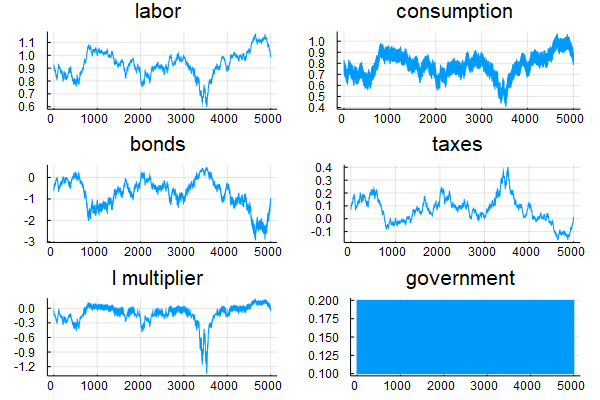
\includegraphics[width = 0.8\textwidth]{../debt_timeseries_linear.png}
    \caption{Preferences linear in consumption}
\end{figure}

\subsection*{Case 2: Preferences that are concave in both consumption and leisure}
In this case, taxes at least in expected value converges to a near zero value. Consumption is much consistently higher after some time as can be seen below. In fact, this tells us that concavity of preferences in utility takes away the random walk trait of taxes as hypothesized by Barro. Further, we can see that getting Barro's result require stringent assumptions on utility. 

\begin{figure}[h!]
  \centering
  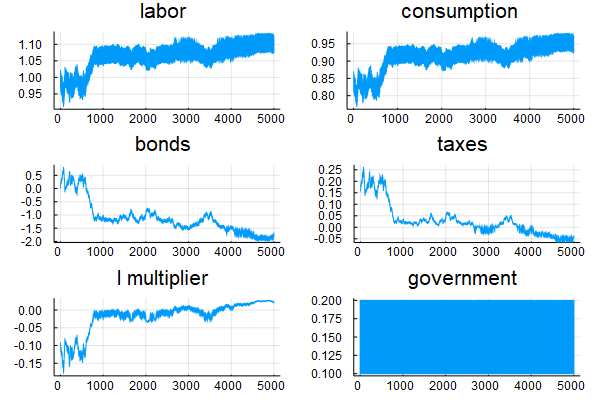
\includegraphics[width = 0.8\textwidth]{../debt_timeseries_concave.png}
    \caption{Preferences linear in consumption}
  \end{figure}

  \section*{Files}
  There are two julia files related to AMSS. One of them is called AMSS.jl and contains all the functions used to solve the model and generate time series for the plots in this document. The other is AMSS\_main.jl which defines parameters and generates the plots. There is one jupyter notebook which is my implementation of LS. In the latex folder there is this file which is my assignment and notes.pdf which is for my own records, but I included here as well.  
\end{document}
